\documentclass[a4paper]{article}

% support for footnote style author/affiliation
\usepackage{authblk}
% typeset source code listings using LaTeX
\usepackage{listings}
% Enhanced support for graphics 
\usepackage{graphicx}
% positions figures at the end of the document
\usepackage[nomarkers]{endfloat}
% Extensive support for hypertext in LaTeX
\usepackage{hyperref}
% Intelligent cross-referencing WARNING: cleverref has to be loaded after hyperref
\usepackage{cleveref} 
% LaTeX support for the Text Companion fonts
\usepackage{textcomp}
% Show "realistic" quotes in verbatim
\usepackage{upquote}
% Layout with zero \parindent, non-zero \parskip
\usepackage{parskip}
% Rotation tools, including rotated full-page floats
\usepackage{rotating}

%% biblatex options
\usepackage[style=nature,
  natbib=true,
  maxnames=2,
  minnames=1,
  sortcites=true,
  backend=biber,
  block=space]{biblatex}

\DeclareNameAlias{default}{last-first}

\addbibresource{dnaseq-pipeline-manual.bib}

% set listing parameters
\lstset{
  language=bash,
  basicstyle=\ttfamily,
  columns=flexible,
  breaklines=true,
  % breakatwhitespace=true
  prebreak=\small\symbol{'134}
  % postbreak=\raisebox{0ex}[0ex][0ex]{\ensuremath{\hookrightarrow\space}}
}

\newcommand{\Rfunction}[1]{{\texttt{#1}}}
\newcommand{\Robject}[1]{{\texttt{#1}}}
\newcommand{\Rpackage}[1]{{\textit{#1}}}
\newcommand{\Rclass}[1]{{\textit{#1}}}

% description labels as texttt
\renewcommand{\descriptionlabel}[1]{\hspace{\labelsep}\texttt{#1}}


\title{The GOSgene WGS analysis pipeline}

\author{Georg W. Otto \thanks{g.otto@ucl.ac.uk}}

\affil{The UCL Institute of Child Health}

\begin{document}

\maketitle

\tableofcontents

\section{Introduction}
\label{sec:introduction}

This is a pipeline for aligning whole-genome sequencing (WGS) reads to
a genome reference and variant calling
(\Cref{fig:sampleAnalysis,fig:cohortAnalysis}). The
alignment parts follows alignment pipeline standards described in
\citep{Regier2018Functionalequivalenceof} and in the github pages of
\href{https://github.com/CCDG/Pipeline-Standardization/blob/master/PipelineStandard.md}{CCDG},
\href{https://github.com/HGSC-NGSI/HgV_Protocol_Descriptions/blob/master/hgv_ccdg_resequencing.md}{Baylor
  HGSC} and the
\href{https://github.com/statgen/docker-alignment}{Center for
  Statistical Genetics} (University of Michigan).

The variant calling and variant refinement part of the pipeline
follows the GATK
\href{https://software.broadinstitute.org/gatk/best-practices/workflow?id=11145}{Best
  Practices}, in particular the
\href{https://github.com/gatk-workflows/broad-prod-wgs-germline-snps-indels/blob/master/PairedEndSingleSampleWf.wdl}{single
  sample} and
\href{https://github.com/gatk-workflows/broad-prod-wgs-germline-snps-indels/blob/master/JointGenotypingWf.wdl}{cohort} workflows.


\section{Pipeline structure}
\label{sec:pipeline-structure}

This pipeline is a python package consisting of scripts to run the
pipeline and a collection of python modules which define classes and
methods (see class diagram xx). It consists of two parts: (1) An
analysis pipeline that works on a per-sample level, aligning and
processing sequencing reads and performing variant calling, resulting
in a single-sample \texttt{GVCF} file
(\cref{fig:sampleAnalysis}). (2) A cohort-level analysis pipeline that
combines \texttt{GVCF} files from a family or cohort and performs
variant recalibration and genotyping (\cref{fig:cohortAnalysis}).


\begin{figure}
  \begin{center}
    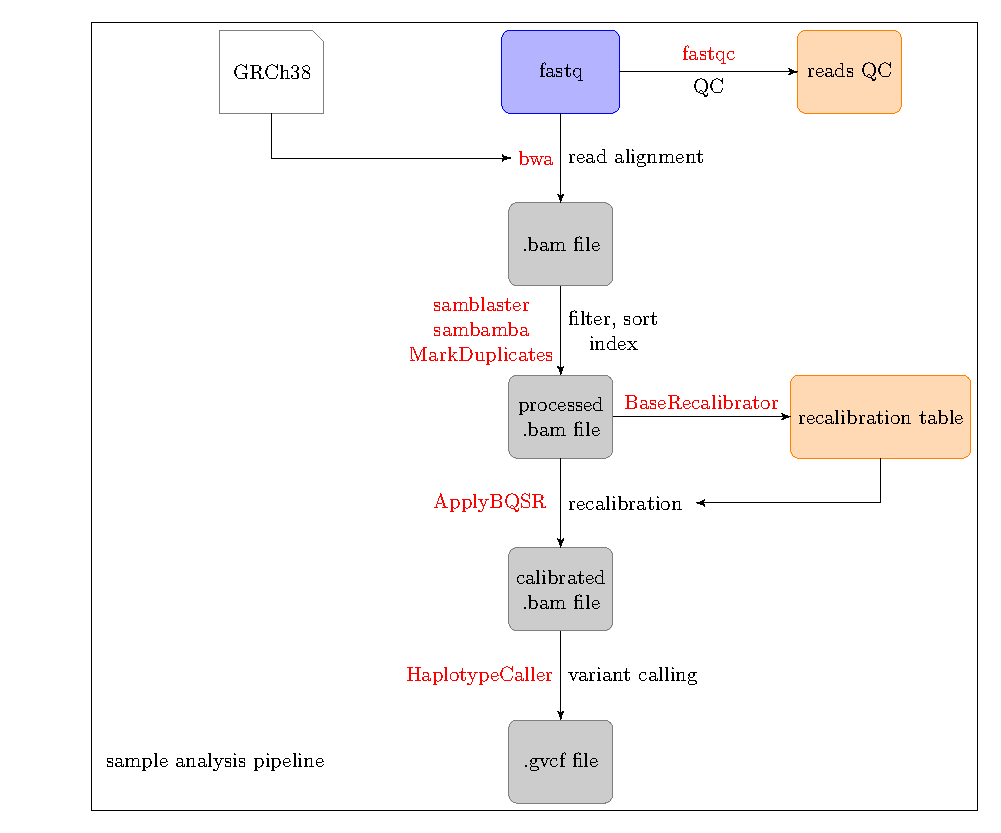
\includegraphics[scale=0.8]{fig-sample-analysis.pdf}
    \caption[sanple analysis]{Flowchart of sample analysis}
  \label{fig:sampleAnalysis}
\end{center}
\end{figure}


\begin{figure}
  \begin{center}
    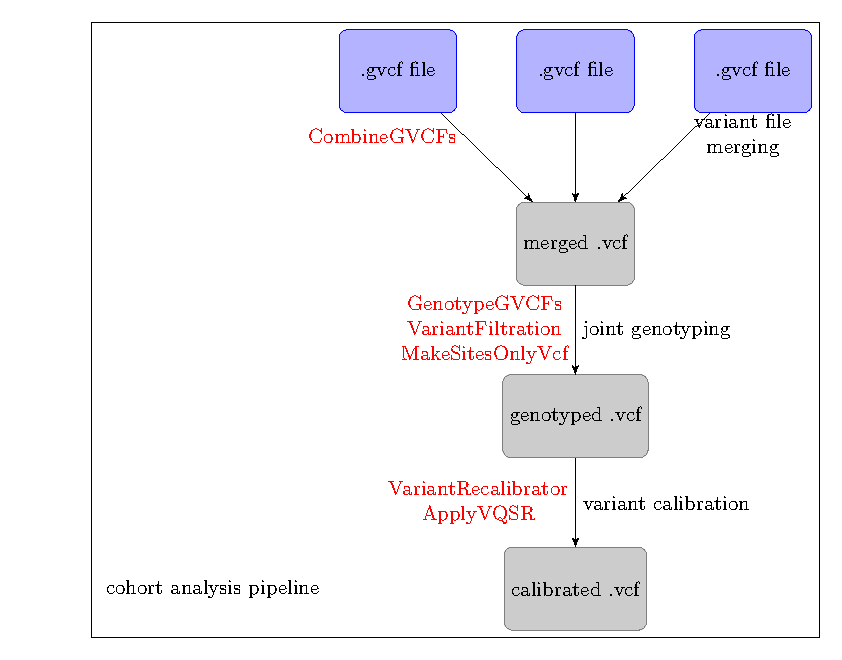
\includegraphics[scale=0.8]{fig-cohort-analysis.pdf}
    \caption[cohort analysis]{Flowchart of cohort analysis}
  \label{fig:cohortAnalysis}
\end{center}
\end{figure}


The pipeline is designed to run on a variety of computing
environments, e.g. on an \texttt{SGE} queueing system or an
interactive shell. I order to achieve this, the pipeline workflows
consist of two levels: Wrapper scripts
(\texttt{initialize\_sample\_analysis.py},
\texttt{initialize\_cohort\_analysis.py}), which take the sample
information from a text file and configurations from a yaml file. They
create the commands, environments and data structures for the pipeline
scripts (\texttt{sample\_analysis.py}, \texttt{cohort\_analysis.py})
and send the jobs to the cluster queue or run them directly as a new
process on the server. This is exemplified in
\Cref{fig:pipelineProcess}.


\begin{enumerate}
\item WGS sample analysis
  \begin{enumerate}
  \item initialization script \texttt{initialize\_sample\_analysis.py}
  \item pipeline script \texttt{sample\_analysis.py}
  \end{enumerate}

\item Cohort analysis
  \begin{enumerate}
  \item initialization script \texttt{initialize\_cohort\_analysis.py}
  \item pipeline script \texttt{cohort\_analysis.py}
  \end{enumerate}

\end{enumerate}


\begin{figure}
  \begin{center}
    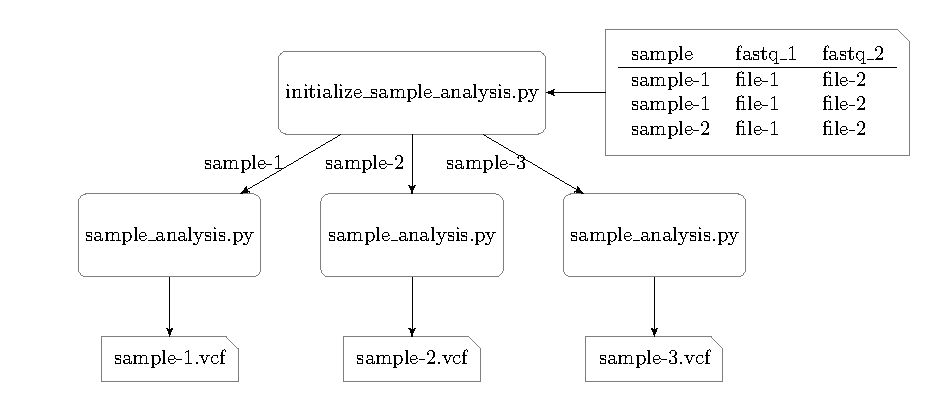
\includegraphics[scale=0.8]{fig-pipeline-structure.pdf}
    \caption[cohort analysis]{Pipeline process deployment}
  \label{fig:pipelineProcess}
\end{center}
\end{figure}



\paragraph{Use of scratch directory}

When running the pipeline on the Computer Science cluster, it is
recommended to move input data to the temporary scratch directory of
each node, and also to write output data there. The pipeline takes
care of the copying of data to and from the scratch directory. In
order to do this, a path to the scratch directory has to be given in
the yaml config file e.g.

\begin{lstlisting}
scratchdir: /scratch0/
\end{lstlisting}

If the scratchdir variable is empty

\begin{lstlisting}
scratchdir: ''
\end{lstlisting}

or has the boolean value \texttt{False}

\begin{lstlisting}
scratchdir: False
\end{lstlisting}

no temporary directory will be used and data are read from and written
to their original location.

\paragraph{Use of environment modules}

The pipeline supports the use of environment modules to control to
load the programs used in the path. This is configured in the
configuration file. There is an option \texttt{modules}, which can be
set to \texttt{False}. In that case environment modules are not used,
and it is assumed that every program needed is in the path.

\section{The WGS sample analysis pipeline}
\label{sec:wgs-sample-analysis}

\subsection{WGS sample analysis initialization}
\label{sec:wgs-sample-analysis-1}


The sample analysis pipeline (\Cref{fig:sampleAnalysis}) is
initialized and started by the command

\begin{lstlisting}
initialize_sample_analysis.py --config-file <file> --run-mode <mode>
\end{lstlisting}

The command line options are:

\begin{description}
\item[--config-file, -c] [mandatory] the path to the yaml
  configuration file containing parameters how to run the pipeline. A
  sample configuration file can be found in
  \texttt{config/config-sample-analysis.yml}. Please copy this file
  and modify it according to your needs.
\item[--run-mode, -r] [optional, default: test] The pipeline can be
  run in different run modes, these are 

  \begin{description}
  \item[test] dry run without initializing the
    \texttt{sample\_analysis.py} program. Prints out the command
    that would be send to the cluster queue.
  \item[server] starts \texttt{sample\_analysis.py} for each
    sample as a subprocess on the machine the wrapper script is
    running.
  \item[cluster] sends a command for each sample to the cluster queue
    in order to run \texttt{sample\_analysis.py}.
  \end{description}
    
\item[--help, -h] [optional] prints a short message containing the
  vailable command line options.
\end{description}


\paragraph{Auxiliary files needed}

\begin{description}

\item[samples-file] A tab-delimited text file, (containing one header
  line). It containes \texttt{fastq} file annotations, with each line
  representing a \texttt{fastq} file or (in case of paired-end
  sequencing) a \texttt{fastq} file pair. The table can contain any
  number of columns, but the components processed by the pipeline are
  the first two or three columns: The first column is the sample
  name. A sample name can occur in multiple lines, because a sample
  can have multiple \texttt{fastq} files or file pairs. All
  \texttt{fastq} files with the same sample name, i.e. read pairs and
  technical replicates, will be combined in the same bam file. The
  second column is the file name of the \texttt{fastq} file in case of
  single end sequencing or of the forward \texttt{fastq} file in case
  of paired-end sequencing. The third column is the file name of the
  \texttt{fastq} reverse file (unique) in case of paired-end
  sequencing.

  example \texttt{data/samples.txt}:

  {\scriptsize
    {\ttfamily
      \begin{tabular}{lll}
        
        sample & fastq\_1 & fastq\_2 \\
        sample-1 & sample-1\_1\_R1.fastq.gz & sample-1\_1\_R2.fastq.gz \\
        sample-1 & sample-1\_2\_R1.fastq.gz & sample-1\_2\_R2.fastq.gz \\
        sample-1 & sample-1\_3\_R1.fastq.gz & sample-1\_3\_R2.fastq.gz \\
        sample-2 & sample-2\_1\_R1.fastq.gz & sample-2\_1\_R2.fastq.gz \\
        sample-2 & sample-2\_2\_R1.fastq.gz & sample-2\_2\_R2.fastq.gz \\
        sample-2 & sample-2\_3\_R1.fastq.gz & sample-2\_3\_R2.fastq.gz \\

      \end{tabular}
    }
  }

  The path to the samples file is set in the configuration file in the
  variable \texttt{samples-file}.

\end{description}

\subsection{The sample analysis pipeline}
\label{sec:sample-analys-pipel-1}

Usually, the sample analysis pipeline is started by the
\texttt{initialize\_sample\_analysis.py} script (section
\ref{sec:wgs-sample-analysis-1}). However the pipeline can be started
directly (for example for tests) for a single sample using the
command:


\begin{lstlisting}
sample_analysis.py --config-file <file> --fastq-object-file <file> --run-mode <mode>
\end{lstlisting}

The command line options are:

\begin{description}
\item[--config-file, -c] [mandatory] the path to the yaml
  configuration file containing parameters how to run the pipeline. A
  sample configuration file can be found in
  \texttt{config/config-sample-analysis.cfg}. Please copy this file
  and modify it according to your needs.
\item[--fastq-object-file, -f] the path to a file containing the
  serialized \texttt{Fastq} object of the sample, in \texttt{pickle}
  format.
\item[--run-mode, -r] [optional, default: test] The pipeline can be
  run in different run modes, these are 

  \begin{description}
  \item[test] for debugging, does not delete the input \texttt{.pkl}
    file and does not delete the scratch directory upon pipeline
    completeion.
  \item[server] configurations for running the pipeline directly on
    the server where it is invoked (e.g. not in a cluster queue).
  \item[cluster] configurations for queuing and running the pipeline
    on a sge cluster.
  \end{description}
    
\item[--help, -h] [optional] prints a short message containing the
  vailable command line options.

\item[--version, -v] [optional] prints the version of the pipeline.

\end{description}


\section{The WGS cohort analysis pipeline}
\label{sec:wgs-cohort-analysis}


\subsection{WGS cohort analysis initialization}
\label{sec:wgs-cohort-analysis-1}


The cohort analysis pipeline (\Cref{fig:cohortAnalysis}) is
initialized and started by the command

\begin{lstlisting}
initialize_cohort_analysis.py --config-file <file> --run-mode <mode>
\end{lstlisting}

The command line options are:

\begin{description}
\item[--config-file, -c] [mandatory] the path to the yaml
  configuration file containing parameters how to run the pipeline. A
  sample configuration file can be found in
  \texttt{config/config-cohort-analysis.yml}. Please copy this file
  and modify it according to your needs.
\item[--run-mode, -r] [optional, default: test] The pipeline can be
  run in different run modes, these are 

  \begin{description}
  \item[test] dry run without initializing the
    \texttt{cohort\_analysis.py} program. Prints out the command
    that would be send to the cluster queue.
  \item[server] starts \texttt{cohort\_analysis.py} for each
    sample as a subprocess on the machine the wrapper script is
    running.
  \item[cluster] sends a command for each sample to the cluster queue
    in order to run \texttt{cohort\_analysis.py}.
  \end{description}
    
\item[--help, -h] [optional] prints a short message containing the
  vailable command line options.
  
\end{description}


\paragraph{Auxiliary files needed}

\begin{description}

\item[cohorts-file] A tab-delimited text file, with sample annotations
  (containing one header line). The table can contain any number of
  columns, but the components processed by the pipeline are the first
  two columns: The first column is the cohort name, the second column
  is the name of the corresponding sample \texttt{GVCF} files. A
  cohort can consist of one or (usually) more samples.

  example \texttt{data/cohorts.txt}:

  {\scriptsize
    {\ttfamily
      \begin{tabular}{ll}

        cohort & vcf \\
        cohort-1 & sample-1.vcf.gz \\
        cohort-1 & sample-2.vcf.gz \\
        cohort-2 & sample-3.vcf.gz \\
        cohort-2 & sample-4.vcf.gz \\
      \end{tabular}
    }
  }

  The path to the samples file is set in the configuration file in the
  variable \texttt{cohorts-file}.

\end{description}

\subsection{The cohorts analysis pipeline}
\label{sec:cohorts-analys-pipel-1}

Usually, the cohorts analysis pipeline is started by the
\texttt{initialize\_cohorts\_analysis.py} script (section
\ref{sec:wgs-cohort-analysis-1}). However the pipeline can also be
started directly (for example for tests) for a single sample using the
command:

\begin{lstlisting}
cohort_analysis.py --config-file <file> --fastq-object-file <file> --run-mode <mode>
\end{lstlisting}

The command line options are:

\begin{description}
\item[--config-file, -c] [mandatory] the path to the yaml configuration
  file containing parameters how to run the pipeline. A sample
  configuration file can be found in
  \texttt{config/config-cohort-analysis.yml}. Please copy this file and
  modify it according to your needs.
\item[--vcf-object-file, -f] the path to a file containing the
  serialized \texttt{Vcf} object of the cohort, in \texttt{pickle}
  format.
\item[--run-mode, -r] [optional, default: test] The pipeline can be
  run in different run modes, these are 

  \begin{description}
  \item[test] for debugging, does not delete the input \texttt{.pkl}
    file and does not delete the scratch directory upon pipeline
    completion.
  \item[server] configurations for running the pipeline directly on
    the server where it is invoked (e.g. not in a cluster queue).
  \item[cluster] configurations for queuing and running the pipeline
    on a sge cluster.
  \end{description}
    
\item[--help, -h] [optional] prints a short message containing the
  vailable command line options.

\item[--version, -v] [optional] prints the version of the pipeline.

\end{description}




\section{Getting help}
\label{sec:getting-help}


Help on how to run the higher level
scripts \texttt{initialize\_sample\_analysis.py} and
\texttt{sample\_analysis.py} can be found using the options
\texttt{-h} or \texttt{--help}:

\begin{verbatim}
python initialize_sample_analysis.py --help
\end{verbatim}

Classes and methods are documented using docstring, so for example to
get documentation of the fastq module, the Fastq class and the
fastqList method of the Fastq class, use:

\begin{verbatim}
import fastq
help(fastq)
help(fastq.Fastq)
help(fastq.Fastq.fastqList)
\end{verbatim}


\subsection{Tests}
\label{sec:tests}

How to run tests


\printbibliography

\end{document}

%%% Local Variables:
%%% mode: latex
%%% TeX-master: t
%%% End:
